\chapter{恒星内部}
\section{描述恒星模型的方程}
研究恒星时,为了简便起见,我们通常把恒星看成是球对称分布的,因此只要研究简单的径向一维模型即可,然后辅以一下方程求解恒星的不同物理量

\paragraph{流体静力学平衡}
恒星要保持稳定结构,需要内部足够的压强梯度来平衡自身的引力,防止塌缩。
\begin{equation}
  \underbrace{dP\over dr}_\text{压强梯度力}=\underbrace{-G{M_r \rho\over r^2}}_\text{引力}=-\rho g
\end{equation}

\paragraph{物态方程}
描述压强与温度的关系
\begin{equation}
  \begin{dcases}
    P_g={\rho \over \mu m_H}kT\qquad\text{理想气体压强}\\
    P_\mathrm{rad}={1\over3}aT^4\qquad\text{辐射压}
  \end{dcases}
\end{equation}


\paragraph{质量守恒方程}
描述质量分布
\begin{equation}
  {dM_r\over dr}=4\pi r^2 \rho
\end{equation}


其中$\mu$为\textbf{平均分子质量},定义为:
\begin{equation}
  \mu\equiv {\bar m \over m_H}\simeq {1\over \displaystyle 2X+{3\over 4}Y+\langle{1+z\over A}\rangle_i Z}
\end{equation}

其中$X$,$Y$,$Z$分别为氢、氦、金属元素的质量分数

\paragraph{能量守恒方程}
描述光度分布
\begin{equation}
  \underbrace{dL_r \over dr}_\text{\clap{光度梯度}}=4\pi r^2\rho \underbrace{\epsilon}_\text{\clap{单位质量产能率}}
\end{equation}

\paragraph{能量转移方程}
描述能量传递过程
\begin{equation}
  {dT\over dr}=
  \begin{dcases}
    -{3\over 4ac}{\bar \kappa \rho \over T^3}{L\over 4\pi r^2}\qquad \text{辐射传能}\\[2mm]
    -\left(1-{1\over \gamma}\right){\mu m_H\over k}{GM_r\over r^2}\qquad \text{对流传能}
  \end{dcases}  
\end{equation}

\section{恒星能量来源}
从人类诞生开始,太阳每时每刻都在辐射巨大的能量,因此人们一度好奇是什么提供太阳能够如此挥霍,太阳的能量来源是什么。最早的方案是太阳塌缩所释放的引力势能,并计算相应的\textbf{热力学时标(开尔文-亥姆霍兹时标)}:
\begin{equation}
  \tau_\mathrm{KH}={\Delta E\over L_\odot}={\displaystyle{3\over10}{GM^2_\odot \over R_\odot}\over L_\odot}\sim10^7\;\mathrm{yr}
\end{equation}

即假设太阳一直以目前的光度辐射,它的总引力势能够它挥霍多少年。计算结果发现只有千万年量级,而当时考古发现的化石年龄已经有数十亿年,难道地球形成比太阳还早?显然不太可能,因此有人的注意力转向了核能,并计算了\textbf{核反应时标}:
\begin{equation}
  \tau_\mathrm{nuc}={\Delta E\over L_\odot}={\phi f_\mathrm{nuc}M_\odot c^2 \over L_\odot}\sim10^10\;\mathrm{yr}
\end{equation}

这种方案假设太阳总质量的一定比例$f_\mathrm{nuc}=70\%$发生核反应,反应效率$\phi=0.007$,计算表明这些能量足够挥霍一百亿年!靠谱!

\paragraph{量子隧穿}
恒星中主要是核聚变,其本质是把两个原子核黏在一块形成更重的原子核,但是原子核带正电,两个原子核要靠近必须要克服它们之间的库伦势垒。不幸的是,库伦力和距离平方成反比,越靠近斥力越大!幸运的是,前面提到了量子隧穿(\ref{uncertainty}节),使得两个原子核有一定几率可以靠近,而隧穿的几率与原子核的内能相关,也就是和温度相关,当几率大到足够产生稳定的核反应时,对应的温度即为\textbf{核点燃温度}:
\begin{equation}
  T_\mathrm{quantum}={\displaystyle Z_1^2 Z_2^2 e^4 \mu_m \over \displaystyle 12\pi^2 \epsilon^2_0 h^2 k}
\end{equation}

对于两个氢原子,平均分子质量$\mu_m=m_p/2$(因为电离),原子序数$Z_1=Z_2=1$(对应核电荷数),$T_\mathrm{quantum}\sim10^7\;\mathrm K$。

\paragraph{伽莫夫峰}
隧穿几率越大,核反应的效率就越高,显然我们能想到核反应速率随原子能量的线性增长。但是由于热平衡系统的粒子速率分布满足麦克斯韦-玻尔兹曼速率分布,高能区域的粒子数量往往会比较少。因此总体来说,如图\ref{fig:gamow},能量太低隧穿几率极低,能量太高的粒子数量极少,真正高效的反应区域是在中间,形成\textbf{伽莫夫峰}。

\begin{figure}[hbt]
  \centering
  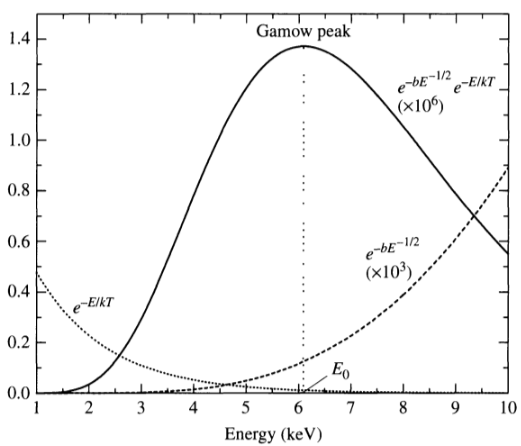
\includegraphics[width=5.6cm]{chapters/10/gamowpeak}
  \caption{核反应可能性示意图。伽莫夫峰是隧穿几率和麦克斯韦-玻尔兹曼速率分布共同作用的结果}
  \label{fig:gamow}
\end{figure}

\newpage
\subsection{核反应类型}
\paragraph{p-p链}
由$^1$H反应生成$^4$He,产能率$\epsilon_{pp}\propto T_6^4$。
\begin{figure}[hbt]
  \centering
  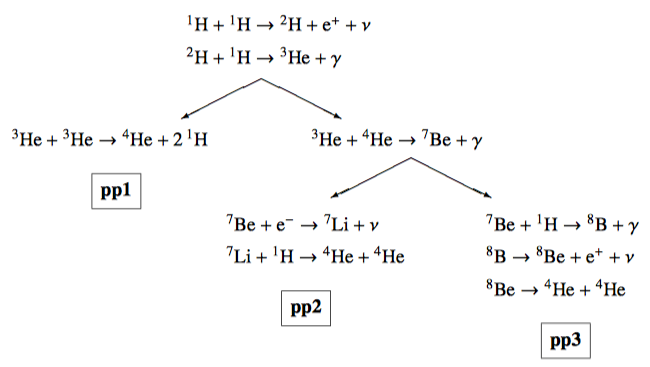
\includegraphics[width=11cm]{chapters/10/ppchains}
  \label{}
\end{figure}


\paragraph{CNO循环}
也是生成$^4$He的核反应,需要温度更高,但是反应更高效,产能率$\epsilon_{CNO}\propto T_6^{19.9}$
\begin{figure}[hbt]
  \centering
  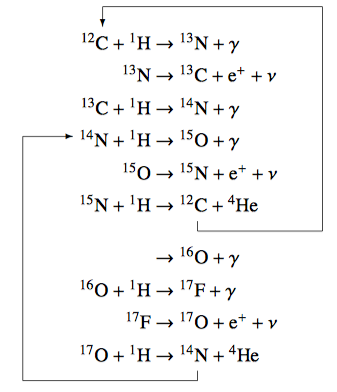
\includegraphics[width=6cm]{chapters/10/cno}
  \label{}
\end{figure}

\paragraph{3$\alpha$反应}
由$^4$He反应生成$^{12}$C,产能率$\epsilon_{3\alpha}\propto T_8^{41}$
\begin{figure}[hbt]
  \centering
  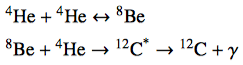
\includegraphics[width=5cm]{chapters/10/3alpha}
  \label{}
\end{figure}



\paragraph{碳氧燃烧}
$^{12}$C和$^{16}$O继续燃烧,生成质量更大的核素\\
\newline
\textcolor{red}{\bf 以上核反应都有各自的点燃温度,温度达到就会开始反应,并且反应速率从上到下关于温度变化越来越敏感}

\begin{figure}[hbt]
  \centering
  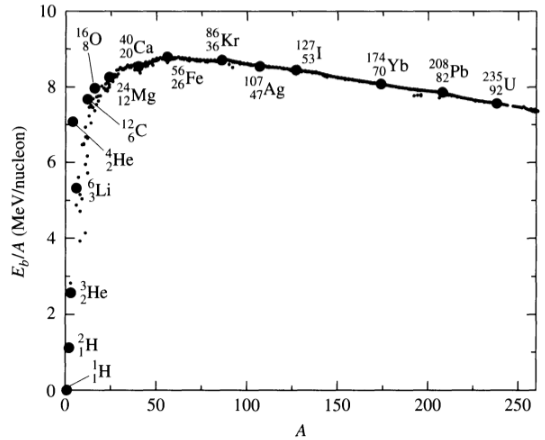
\includegraphics[width=10cm]{chapters/10/bindingenergy}
  \caption{单位核子的结合能。从图中可以看出,铁的位于最大值,铁如果继续聚变生成更重核素就是吸热反应,吸热反应无法在恒星内部自发稳定形成}
  \label{}
\end{figure}



\section{能量转移}
中学时期我们就学过,热传递的三种方式:热传导、热辐射、热对流,能量的传递也是同样的方式
\begin{itemize}
  \item 传导,通过粒子碰撞来传递能量,非常低效,通常在恒星内部不考虑
  \item \textbf{辐射},光子携带能量出去,通过与物质相互作用传递能量
  \item \textbf{对流},通过物质交换形式传递能量,非常高效。但\textbf{产生需满足辐射温度梯度大于绝热温度梯度},即$\nabla_\mathrm{rad}>\nabla_\mathrm{ad}$
\end{itemize}

\paragraph{爱丁顿极限}
当恒星的光度足够大时,光子产生的辐射压在对抗引力的过程中就会占据主导,如果光度继续增加,就会将恒星的物质吹跑,因此这时的光度是恒星能够维持流体静力学平衡的最大光度,称为\textbf{爱丁顿光度},可以通过辐射压与引力平衡计算得到:
\begin{equation}
  L_\mathrm{Ed}={4\pi Gc \over \bar\kappa}M
\end{equation}

\paragraph{沃格特-罗素定理(Vogt-Russel theorem)}
恒星的质量和成分结构就决定了它的半径、光度、内部结构以及未来的演化。
